\chapter{OPTO22}

\section{Introduction}
The process control laboratory has been set up with a number of experimental setups to demonstrate control principles.  These rigs are fitted with analogue process control equipment which can be used to control the processes involved.  If a computer is to be used to control the rigs, a conversion between the analogue data of the rig and the digital data of the computer must be done.  Many attempts have been made to solve this problem, with varying degrees of success.  

In addition, this approach has the disadvantage that a lot of time is spent 'reinventing the wheel' by setting up interfacing hardware and software, as well as being a less realistic image of practical control system monitoring in the field.

Interfacing with the process equipment should be less about hardware needed between the process and the computer than the actual work done on these components.  A new system removing the wiring from the process is proposed in this document, along with the requirements to be complied with to enjoy the full benefits of this system on each setup.

\section{Problem statement}
The problem of interfacing with the laboratory equipment can be broken into four parts, which will be discussed separately.  The equipment will be referred to as `rigs' and the `user' will be the person or system accessing the rigs.
\subsection{Physical interfacing}
Each element that needs to be accessed has to be physically connected to the user in some way.  The connection must be 
\begin{itemize}
	\item reliable,
	\item noise free and
	\item easily maintained.
\end{itemize}
	
\subsection{Conversion}
Conversion from analogue to digital (A/D) and from digital to analogue (D/A) signals is required.  Each experimental setup accepts analogue signals to control valves and other final control elements.  Measuring devices on the rigs return analogue data that has to be converted to digital signals for computer based control.

\subsection{Data Storage}
Data collected from the various rigs should be stored and accessible for a time period after experiments have been carried out on them.  This will enable users to do experiments without manually logging results or writing their own logging procedures.

\subsection{Software Interfacing}
All the above requirements are dedicated to providing process data and control handles to control software.  The collected and stored data must be accessible from many environments such as MATLAB and HISYS.  

\section{Conceptual design}
\subsection{General}

Conceptually, the system includes wiring to and from all the units, connected to a central bank of A/D and D/A converters connected to a central data server.  The values will be accessed using a tag system similar to SCADA systems.

The components identified above and the relationships between them are shown in Figure~\ref{fig:SCADAoverview}.

\begin{figure}
	\centering
	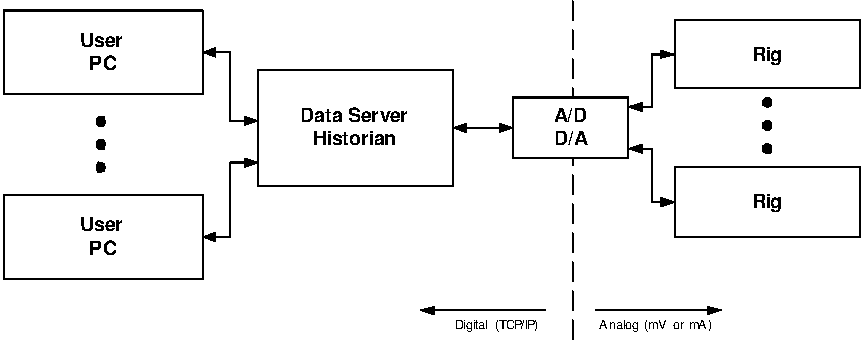
\includegraphics[width=\fullwidth]{SCADAoverview}
	\caption[Conceptual SCADA layout]{Conceptual layout of the SCADA system.  Signals to the left of the A/D-D/A line are digital, while signals to the right are analog.}
	\label{fig:SCADAoverview}
\end{figure}

It should be clear from the figure that the user does not have direct access to the analogue data, and that the server acts as an abstraction layer between the converter and the computer user.  This enables the user to focus on the design of a control system instead of worrying about the mechanics of A/D. It also protects the user from short circuits and other analogue errors on the rig.

The wiring from the experimental setup terminates in a junction box.  This junction box (JB) serves as the physical connection point between the system and the experimental setup.  It should be possible to do most of the maintenance required for each rig without ever opening the central converter's box. 

In addition to the signal interfacing, the JB should provide space for power converters as required by each rig.  This ensures that the rigs do not have high voltage power open to spills and accidental touch.

\subsection{Software interface}
The server computer will have to run software that is capable of data storage and retrieval.  Possibly a general web interface could be included.  This software should include methods to interface with the A/D converter.

\subsection{Documentation}
Documenting a complex system such as this one is challenging for the user.  A system will have to be put in place that removes most of the possibility for error.  A database system for tracking connections and changes in the rigs required.  Diagram standards for wiring and rig setups are also needed.

\section{Detail design}
\subsection{Physical interfacing}
Wiring from the central conversion unit to each of the rigs will consist of shielded single twisted pair wires.  Each wire represents a signal, using the two conductors in the wires to transfer it.  The shielding ensures that signal quality is preserved. 

Each rig is fitted with a junction box (JB), where the wiring from the central point terminates in connectors.  These connectors provide a convenient connection point for signals from the rigs, while the JB itself provides a safe environment for the open terminals and power supply units.  

Mild steel junction boxes with polycarbonate viewing windows are used.  Junction boxes are specified to IP55 standard, ensuring protection from dust and spills on the rigs.

Based on the amount of signals to and from each rig, a size of 400$\times$300$\times$120mm was chosen, with DIN rail mounted connectors.  Power supplies were added into the size calculations, as these should also be in the JB.

\subsection{Conversion}
The OPTO22 system will be used to handle conversion.  This system operates on an attractive modular principle, which includes conversion to and from many different analog and digital signals.  Conversion modules called SNAP modules are connected to a rack with a 'brain' unit which transfers information to the network using TCP/IP.  Information was obtained from OPTO22 (form 1112).

OPTO22 SNAP Ethernet brains are compact, flexible high performance processors for many applications.  The SNAP-B3000-ENET brain was chosen, as this is the baseline brain and complies with all the requirements while being the cheapest of the SNAP brains.  Two units are required for the signals currently used in the laboratory.

Each rack has room for 12 modules.  These may include the following convertor modules:
\begin{itemize}
	\item	AIMA-4: $\pm$20mA input (A/D)
	\item	AITM:  Thermocouple input (A/D)
	\item	AOA-23: 4-20mA output (D/A)
\end{itemize}

The OPTO22 units will be installed in a junction box of the same specifications as the rig JBs, but with the larger dimension of 800$\times$600$\times$210mm.  The OPTO22 housing design can be seen in Appendix A.

\subsection{Data storage and software interfacing}
Mintek has produced a SCADA-like system called PlantStar.  PlantStar, installed on a server connected to the OPTO22 box will manage data collection and retrieval.  Plantstar includes a web-based interface for monitoring and basic control.  Connections to other programs are possible using calls to the client application installed on user PCs.

The system has to be installed on a computer running Microsoft Windows 2000, with a large hard drive and more than 128MB of RAM.  A 13GB hard drive will be installed for data storage.

\subsection{Documentation}
The wiring system has many connections and tag numbers.  A systematised method is required to keep track of thes numbers.
\subsubsection{Tags}
Tag numbers conform to ISA standards.  Tags are built as follows:\bigskip

\begin{centering}
	\framebox{Rig number} -- \framebox{Object type code} -- \framebox{Object number} \bigskip \\
\end{centering}

Rig numbers are two digits padded with a leading zero if required.  Object numbers are three digits with leading zeros and increment sequentially from 001 for each unique object type on a rig.  Rig numbers and current object type codes can be found in appendix A.  These lists are dynamic, allowing for expansion of the rigs and labs.

\subsubsection{Wire names}
Wire names are generated from the numbers of the connectors the wires connect. \bigskip

\begin{centering}
\framebox{Rig connector number}  / \framebox{OPTO connector number} \bigskip \\
\end{centering}

Where both numbers are three digits padded with leading zeros.  These numbers are affixed to the wire so that they are legible when read in a direction from the rigs to the OPTO JB.

\subsubsection{Diagrams}
Three types of wiring diagrams are needed for documentation of the system:
\begin{itemize}
	\item	JB Box layout diagrams,
	\item	loop diagrams and
	\item	rig PIDs.
\end{itemize}

Diagrams for the distillation column have been drawn up and can be seen in appendix B.

\subsubsection{Equipment Database}
To simplify the documentation of the wiring and connectors, an equipment database is required.  This database tracks each piece of process control equipment and the connections between them.
The starting point for the database is the rig table, which contains the number and name of all the rigs.  From here, linked to the rig number an equipment table stores each item's type and number.  In addition, data is stored about the date of acquisition and origin of the equipment to simplify maintenance and reordering.  To make the database extendable, a table of equipment types is linked to the equipment table, storing the tag extension of the equipment type. 

Queries are defined to generate tag numbers in accordance with the standards set out above, by combining the rig number, equipment type extension and the equipment number.

In order to track connections, each equipment record also stores the unique ID of another piece of equipment.  The direction of this linked list is defined as away from the final control elements and measuring devices.  Therefore, a control valve will link to the JB connector and an OPTO snap in module will link to the OPTO JB connector.  JB connectors reference one another.  This means that the wires connecting JB connectors on both the rig and OPTO side can be traced by following the links from either side.

Wire names are generated by a SQL query, adding the numbers from the connected pieces of equipment.  A list of wire names can be drawn up in a report for wire checking.

\subsection{New equipment}
To keep the documentation current, the following steps are required when adding new equipment.

\begin{description}
\item[Step 1] Collect information
The following information is pertinent when installing new equipment:
\begin{itemize}
	\item	What type of signal does the equipment send or receive?  This will determine the module on the OPTO that the equipment will be wired to.
	\item	Are there enough connectors in the JBs to accommodate the new signal?  If not, new connectors must be installed.
	\item	Are there enough OPTO modules of the type required? If not, a new OPTO module must be installed.
\end{itemize}

\item[Step 2] Add the equipment to the equipment database.
Check that the equipment type exist by double clicking the equipment type table.  If the equipment type does not exist, add a new type on the last line of the table and close the table view.  Open the equipment table by double clicking it.  Select the rig and equipment type from the drop down list.  Enter a unique number for the equipment in the number field, then select the tag number of the equipment this item is connected to.  For instance, a thermocouple would be connected to a connector in the JB for the rig.
If there are no free connectors in the JB, follow the same steps as above for two new connectors: one in the rig JB and one in the OPTO JB.

\item[Step 3] Lay the wiring
Open the trunking and lay a new wire between the OPTO JB and the rig JB, bearing in mind that the wire must be labelled with its wire number.  Use the wire number for the wire between the connectors mentioned above.  This number is generated automatically by the database in the wire numbers query.

\item[Step 4] Connect the wires
The wires are now connected between connectors

\item[Step 5] Test
Before the equipment is used, a signal check must be run.  Using a Ohmmeter, check the resistance between the terminals of the new signal.  This should be very high.  Low values indicate a short circuit.

\item[Step 6] Connect equipment and OPTO
The wires are now connected to the equipment and to the OPTO module.
\end{description}

\section{Conclusion}
The process control laboratories have been fitted with a well designed solution to interfacing with process equipment.  Extensive document standards and the database structure that has been developed make the maintenance of the system efficient and reduces errors.  The PlantStar software used in conjunction with the OPTO22 system provides reliable centralised A/D conversion and data logging facilities.  The software also makes provision for snap in modules that can implement additional data tasks.

\section{Recommendations}
Further investigation into the OPC interface is recommended to connect more programs to the system.  Specifically, an interface to MATLAB must be developed in order for users to interface MATLAB control algorithms with their rigs.  It is also recommended that the rigs be upgraded using standard equipment in order to facilitate modular layout of rigs.

Thought should be given to the virtual connection of rigs via the data server, allowing more complex control problems to be tackled.

Software development recommended include an interface for the database which makes it more user friendly while retaining the functionality of the underlying database.  Additional methods for direct interfacing include an addin for Plantstar which will do calibration of thermocouples and pH probes.
